% Created by tikzDevice version 0.12 on 2019-04-19 15:01:48
% !TEX encoding = UTF-8 Unicode
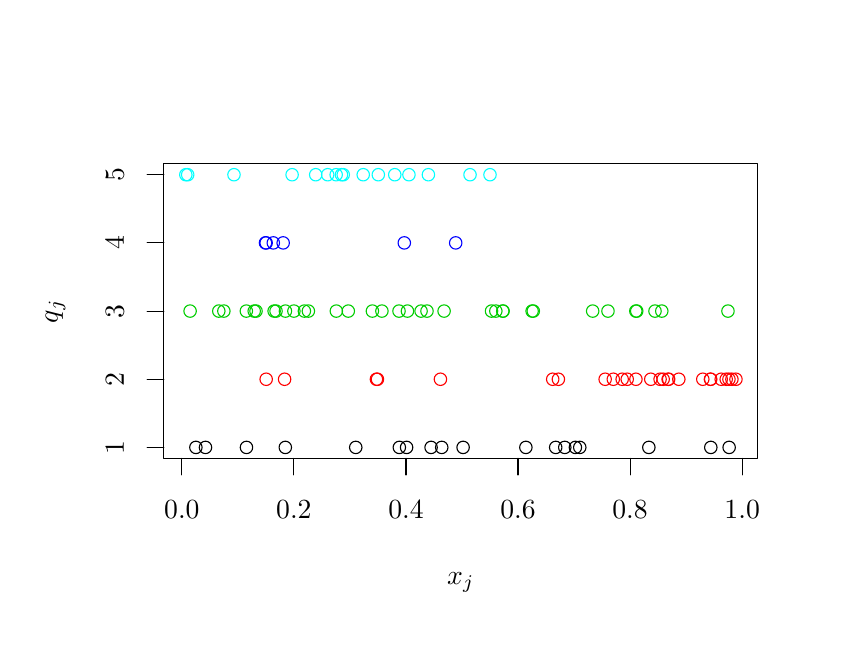
\begin{tikzpicture}[x=1pt,y=1pt]
\definecolor{fillColor}{RGB}{255,255,255}
\path[use as bounding box,fill=fillColor,fill opacity=0.00] (0,0) rectangle (289.08,216.81);
\begin{scope}
\path[clip] ( 49.20, 61.20) rectangle (263.88,167.61);
\definecolor{drawColor}{RGB}{0,205,0}

\path[draw=drawColor,line width= 0.4pt,line join=round,line cap=round] ( 93.14,114.40) circle (  2.25);
\definecolor{drawColor}{RGB}{0,0,0}

\path[draw=drawColor,line width= 0.4pt,line join=round,line cap=round] (197.92, 65.14) circle (  2.25);
\definecolor{drawColor}{RGB}{0,205,0}

\path[draw=drawColor,line width= 0.4pt,line join=round,line cap=round] (171.79,114.40) circle (  2.25);

\path[draw=drawColor,line width= 0.4pt,line join=round,line cap=round] ( 89.74,114.40) circle (  2.25);
\definecolor{drawColor}{RGB}{255,0,0}

\path[draw=drawColor,line width= 0.4pt,line join=round,line cap=round] (246.81, 89.77) circle (  2.25);

\path[draw=drawColor,line width= 0.4pt,line join=round,line cap=round] (246.73, 89.77) circle (  2.25);
\definecolor{drawColor}{RGB}{0,205,0}

\path[draw=drawColor,line width= 0.4pt,line join=round,line cap=round] ( 81.86,114.40) circle (  2.25);
\definecolor{drawColor}{RGB}{0,0,0}

\path[draw=drawColor,line width= 0.4pt,line join=round,line cap=round] (224.46, 65.14) circle (  2.25);
\definecolor{drawColor}{RGB}{0,205,0}

\path[draw=drawColor,line width= 0.4pt,line join=round,line cap=round] (150.47,114.40) circle (  2.25);
\definecolor{drawColor}{RGB}{0,255,255}

\path[draw=drawColor,line width= 0.4pt,line join=round,line cap=round] (167.06,163.67) circle (  2.25);
\definecolor{drawColor}{RGB}{0,205,0}

\path[draw=drawColor,line width= 0.4pt,line join=round,line cap=round] (167.61,114.40) circle (  2.25);
\definecolor{drawColor}{RGB}{0,255,255}

\path[draw=drawColor,line width= 0.4pt,line join=round,line cap=round] (104.08,163.67) circle (  2.25);
\definecolor{drawColor}{RGB}{0,205,0}

\path[draw=drawColor,line width= 0.4pt,line join=round,line cap=round] (209.69,114.40) circle (  2.25);
\definecolor{drawColor}{RGB}{0,0,255}

\path[draw=drawColor,line width= 0.4pt,line join=round,line cap=round] ( 92.32,139.04) circle (  2.25);
\definecolor{drawColor}{RGB}{0,255,255}

\path[draw=drawColor,line width= 0.4pt,line join=round,line cap=round] (137.77,163.67) circle (  2.25);
\definecolor{drawColor}{RGB}{255,0,0}

\path[draw=drawColor,line width= 0.4pt,line join=round,line cap=round] (228.52, 89.77) circle (  2.25);

\path[draw=drawColor,line width= 0.4pt,line join=round,line cap=round] (253.40, 89.77) circle (  2.25);
\definecolor{drawColor}{RGB}{0,205,0}

\path[draw=drawColor,line width= 0.4pt,line join=round,line cap=round] (101.43,114.40) circle (  2.25);
\definecolor{drawColor}{RGB}{0,0,0}

\path[draw=drawColor,line width= 0.4pt,line join=round,line cap=round] (145.77, 65.14) circle (  2.25);
\definecolor{drawColor}{RGB}{0,205,0}

\path[draw=drawColor,line width= 0.4pt,line join=round,line cap=round] ( 70.89,114.40) circle (  2.25);
\definecolor{drawColor}{RGB}{255,0,0}

\path[draw=drawColor,line width= 0.4pt,line join=round,line cap=round] (189.72, 89.77) circle (  2.25);
\definecolor{drawColor}{RGB}{0,205,0}

\path[draw=drawColor,line width= 0.4pt,line join=round,line cap=round] (134.18,114.40) circle (  2.25);
\definecolor{drawColor}{RGB}{255,0,0}

\path[draw=drawColor,line width= 0.4pt,line join=round,line cap=round] (225.15, 89.77) circle (  2.25);
\definecolor{drawColor}{RGB}{0,0,255}

\path[draw=drawColor,line width= 0.4pt,line join=round,line cap=round] ( 86.18,139.04) circle (  2.25);
\definecolor{drawColor}{RGB}{255,0,0}

\path[draw=drawColor,line width= 0.4pt,line join=round,line cap=round] (126.02, 89.77) circle (  2.25);
\definecolor{drawColor}{RGB}{0,0,255}

\path[draw=drawColor,line width= 0.4pt,line join=round,line cap=round] (154.67,139.04) circle (  2.25);

\path[draw=drawColor,line width= 0.4pt,line join=round,line cap=round] ( 85.93,139.04) circle (  2.25);
\definecolor{drawColor}{RGB}{0,205,0}

\path[draw=drawColor,line width= 0.4pt,line join=round,line cap=round] (128.00,114.40) circle (  2.25);
\definecolor{drawColor}{RGB}{255,0,0}

\path[draw=drawColor,line width= 0.4pt,line join=round,line cap=round] (250.61, 89.77) circle (  2.25);
\definecolor{drawColor}{RGB}{0,205,0}

\path[draw=drawColor,line width= 0.4pt,line join=round,line cap=round] ( 82.51,114.40) circle (  2.25);
\definecolor{drawColor}{RGB}{0,255,255}

\path[draw=drawColor,line width= 0.4pt,line join=round,line cap=round] ( 57.82,163.67) circle (  2.25);
\definecolor{drawColor}{RGB}{0,205,0}

\path[draw=drawColor,line width= 0.4pt,line join=round,line cap=round] ( 89.05,114.40) circle (  2.25);

\path[draw=drawColor,line width= 0.4pt,line join=round,line cap=round] (219.75,114.40) circle (  2.25);
\definecolor{drawColor}{RGB}{255,0,0}

\path[draw=drawColor,line width= 0.4pt,line join=round,line cap=round] (231.62, 89.77) circle (  2.25);
\definecolor{drawColor}{RGB}{0,255,255}

\path[draw=drawColor,line width= 0.4pt,line join=round,line cap=round] (159.84,163.67) circle (  2.25);
\definecolor{drawColor}{RGB}{0,205,0}

\path[draw=drawColor,line width= 0.4pt,line join=round,line cap=round] (182.70,114.40) circle (  2.25);

\path[draw=drawColor,line width= 0.4pt,line join=round,line cap=round] (226.68,114.40) circle (  2.25);
\definecolor{drawColor}{RGB}{0,255,255}

\path[draw=drawColor,line width= 0.4pt,line join=round,line cap=round] (113.39,163.67) circle (  2.25);
\definecolor{drawColor}{RGB}{0,0,0}

\path[draw=drawColor,line width= 0.4pt,line join=round,line cap=round] (190.80, 65.14) circle (  2.25);
\definecolor{drawColor}{RGB}{255,0,0}

\path[draw=drawColor,line width= 0.4pt,line join=round,line cap=round] ( 86.18, 89.77) circle (  2.25);

\path[draw=drawColor,line width= 0.4pt,line join=round,line cap=round] (254.48, 89.77) circle (  2.25);
\definecolor{drawColor}{RGB}{0,205,0}

\path[draw=drawColor,line width= 0.4pt,line join=round,line cap=round] (115.85,114.40) circle (  2.25);

\path[draw=drawColor,line width= 0.4pt,line join=round,line cap=round] ( 79.01,114.40) circle (  2.25);
\definecolor{drawColor}{RGB}{0,0,255}

\path[draw=drawColor,line width= 0.4pt,line join=round,line cap=round] ( 88.75,139.04) circle (  2.25);
\definecolor{drawColor}{RGB}{0,0,0}

\path[draw=drawColor,line width= 0.4pt,line join=round,line cap=round] (246.85, 65.14) circle (  2.25);
\definecolor{drawColor}{RGB}{255,0,0}

\path[draw=drawColor,line width= 0.4pt,line join=round,line cap=round] (216.64, 89.77) circle (  2.25);
\definecolor{drawColor}{RGB}{0,205,0}

\path[draw=drawColor,line width= 0.4pt,line join=round,line cap=round] (253.05,114.40) circle (  2.25);
\definecolor{drawColor}{RGB}{255,0,0}

\path[draw=drawColor,line width= 0.4pt,line join=round,line cap=round] (126.39, 89.77) circle (  2.25);
\definecolor{drawColor}{RGB}{0,0,0}

\path[draw=drawColor,line width= 0.4pt,line join=round,line cap=round] (157.34, 65.14) circle (  2.25);
\definecolor{drawColor}{RGB}{255,0,0}

\path[draw=drawColor,line width= 0.4pt,line join=round,line cap=round] (219.79, 89.77) circle (  2.25);
\definecolor{drawColor}{RGB}{0,255,255}

\path[draw=drawColor,line width= 0.4pt,line join=round,line cap=round] ( 57.15,163.67) circle (  2.25);
\definecolor{drawColor}{RGB}{0,205,0}

\path[draw=drawColor,line width= 0.4pt,line join=round,line cap=round] ( 58.69,114.40) circle (  2.25);
\definecolor{drawColor}{RGB}{0,0,0}

\path[draw=drawColor,line width= 0.4pt,line join=round,line cap=round] (194.08, 65.14) circle (  2.25);
\definecolor{drawColor}{RGB}{255,0,0}

\path[draw=drawColor,line width= 0.4pt,line join=round,line cap=round] (243.95, 89.77) circle (  2.25);
\definecolor{drawColor}{RGB}{0,255,255}

\path[draw=drawColor,line width= 0.4pt,line join=round,line cap=round] (111.47,163.67) circle (  2.25);
\definecolor{drawColor}{RGB}{0,205,0}

\path[draw=drawColor,line width= 0.4pt,line join=round,line cap=round] (220.08,114.40) circle (  2.25);
\definecolor{drawColor}{RGB}{255,0,0}

\path[draw=drawColor,line width= 0.4pt,line join=round,line cap=round] (214.82, 89.77) circle (  2.25);

\path[draw=drawColor,line width= 0.4pt,line join=round,line cap=round] (255.93, 89.77) circle (  2.25);
\definecolor{drawColor}{RGB}{0,0,0}

\path[draw=drawColor,line width= 0.4pt,line join=round,line cap=round] (180.02, 65.14) circle (  2.25);

\path[draw=drawColor,line width= 0.4pt,line join=round,line cap=round] (199.50, 65.14) circle (  2.25);
\definecolor{drawColor}{RGB}{255,0,0}

\path[draw=drawColor,line width= 0.4pt,line join=round,line cap=round] (211.61, 89.77) circle (  2.25);

\path[draw=drawColor,line width= 0.4pt,line join=round,line cap=round] (235.29, 89.77) circle (  2.25);
\definecolor{drawColor}{RGB}{0,205,0}

\path[draw=drawColor,line width= 0.4pt,line join=round,line cap=round] (182.28,114.40) circle (  2.25);
\definecolor{drawColor}{RGB}{0,255,255}

\path[draw=drawColor,line width= 0.4pt,line join=round,line cap=round] (108.41,163.67) circle (  2.25);
\definecolor{drawColor}{RGB}{255,0,0}

\path[draw=drawColor,line width= 0.4pt,line join=round,line cap=round] (229.64, 89.77) circle (  2.25);
\definecolor{drawColor}{RGB}{0,205,0}

\path[draw=drawColor,line width= 0.4pt,line join=round,line cap=round] (144.29,114.40) circle (  2.25);
\definecolor{drawColor}{RGB}{0,0,0}

\path[draw=drawColor,line width= 0.4pt,line join=round,line cap=round] (134.30, 65.14) circle (  2.25);
\definecolor{drawColor}{RGB}{255,0,0}

\path[draw=drawColor,line width= 0.4pt,line join=round,line cap=round] (149.15, 89.77) circle (  2.25);
\definecolor{drawColor}{RGB}{0,205,0}

\path[draw=drawColor,line width= 0.4pt,line join=round,line cap=round] ( 99.99,114.40) circle (  2.25);

\path[draw=drawColor,line width= 0.4pt,line join=round,line cap=round] ( 69.06,114.40) circle (  2.25);

\path[draw=drawColor,line width= 0.4pt,line join=round,line cap=round] (111.53,114.40) circle (  2.25);
\definecolor{drawColor}{RGB}{0,0,0}

\path[draw=drawColor,line width= 0.4pt,line join=round,line cap=round] (118.55, 65.14) circle (  2.25);

\path[draw=drawColor,line width= 0.4pt,line join=round,line cap=round] ( 64.25, 65.14) circle (  2.25);

\path[draw=drawColor,line width= 0.4pt,line join=round,line cap=round] ( 93.10, 65.14) circle (  2.25);
\definecolor{drawColor}{RGB}{255,0,0}

\path[draw=drawColor,line width= 0.4pt,line join=round,line cap=round] ( 92.84, 89.77) circle (  2.25);

\path[draw=drawColor,line width= 0.4pt,line join=round,line cap=round] (208.67, 89.77) circle (  2.25);
\definecolor{drawColor}{RGB}{0,255,255}

\path[draw=drawColor,line width= 0.4pt,line join=round,line cap=round] (114.03,163.67) circle (  2.25);
\definecolor{drawColor}{RGB}{255,0,0}

\path[draw=drawColor,line width= 0.4pt,line join=round,line cap=round] (231.42, 89.77) circle (  2.25);
\definecolor{drawColor}{RGB}{0,205,0}

\path[draw=drawColor,line width= 0.4pt,line join=round,line cap=round] (137.23,114.40) circle (  2.25);

\path[draw=drawColor,line width= 0.4pt,line join=round,line cap=round] (171.66,114.40) circle (  2.25);
\definecolor{drawColor}{RGB}{0,255,255}

\path[draw=drawColor,line width= 0.4pt,line join=round,line cap=round] (126.70,163.67) circle (  2.25);
\definecolor{drawColor}{RGB}{255,0,0}

\path[draw=drawColor,line width= 0.4pt,line join=round,line cap=round] (191.77, 89.77) circle (  2.25);
\definecolor{drawColor}{RGB}{0,0,0}

\path[draw=drawColor,line width= 0.4pt,line join=round,line cap=round] ( 60.78, 65.14) circle (  2.25);

\path[draw=drawColor,line width= 0.4pt,line join=round,line cap=round] (136.92, 65.14) circle (  2.25);
\definecolor{drawColor}{RGB}{0,205,0}

\path[draw=drawColor,line width= 0.4pt,line join=round,line cap=round] ( 96.20,114.40) circle (  2.25);

\path[draw=drawColor,line width= 0.4pt,line join=round,line cap=round] (229.13,114.40) circle (  2.25);
\definecolor{drawColor}{RGB}{255,0,0}

\path[draw=drawColor,line width= 0.4pt,line join=round,line cap=round] (252.41, 89.77) circle (  2.25);
\definecolor{drawColor}{RGB}{0,255,255}

\path[draw=drawColor,line width= 0.4pt,line join=round,line cap=round] (121.25,163.67) circle (  2.25);
\definecolor{drawColor}{RGB}{0,205,0}

\path[draw=drawColor,line width= 0.4pt,line join=round,line cap=round] (204.16,114.40) circle (  2.25);

\path[draw=drawColor,line width= 0.4pt,line join=round,line cap=round] (124.56,114.40) circle (  2.25);
\definecolor{drawColor}{RGB}{0,0,0}

\path[draw=drawColor,line width= 0.4pt,line join=round,line cap=round] (253.47, 65.14) circle (  2.25);
\definecolor{drawColor}{RGB}{0,0,255}

\path[draw=drawColor,line width= 0.4pt,line join=round,line cap=round] (136.09,139.04) circle (  2.25);
\definecolor{drawColor}{RGB}{0,255,255}

\path[draw=drawColor,line width= 0.4pt,line join=round,line cap=round] (132.65,163.67) circle (  2.25);
\definecolor{drawColor}{RGB}{0,205,0}

\path[draw=drawColor,line width= 0.4pt,line join=round,line cap=round] (169.17,114.40) circle (  2.25);
\definecolor{drawColor}{RGB}{0,0,0}

\path[draw=drawColor,line width= 0.4pt,line join=round,line cap=round] (149.62, 65.14) circle (  2.25);
\definecolor{drawColor}{RGB}{0,255,255}

\path[draw=drawColor,line width= 0.4pt,line join=round,line cap=round] ( 95.55,163.67) circle (  2.25);
\definecolor{drawColor}{RGB}{0,205,0}

\path[draw=drawColor,line width= 0.4pt,line join=round,line cap=round] (142.15,114.40) circle (  2.25);
\definecolor{drawColor}{RGB}{0,255,255}

\path[draw=drawColor,line width= 0.4pt,line join=round,line cap=round] ( 74.55,163.67) circle (  2.25);
\definecolor{drawColor}{RGB}{0,0,0}

\path[draw=drawColor,line width= 0.4pt,line join=round,line cap=round] ( 79.06, 65.14) circle (  2.25);
\definecolor{drawColor}{RGB}{0,255,255}

\path[draw=drawColor,line width= 0.4pt,line join=round,line cap=round] (144.80,163.67) circle (  2.25);
\end{scope}
\begin{scope}
\path[clip] (  0.00,  0.00) rectangle (289.08,216.81);
\definecolor{drawColor}{RGB}{0,0,0}

\path[draw=drawColor,line width= 0.4pt,line join=round,line cap=round] ( 55.71, 61.20) -- (258.18, 61.20);

\path[draw=drawColor,line width= 0.4pt,line join=round,line cap=round] ( 55.71, 61.20) -- ( 55.71, 55.20);

\path[draw=drawColor,line width= 0.4pt,line join=round,line cap=round] ( 96.20, 61.20) -- ( 96.20, 55.20);

\path[draw=drawColor,line width= 0.4pt,line join=round,line cap=round] (136.70, 61.20) -- (136.70, 55.20);

\path[draw=drawColor,line width= 0.4pt,line join=round,line cap=round] (177.19, 61.20) -- (177.19, 55.20);

\path[draw=drawColor,line width= 0.4pt,line join=round,line cap=round] (217.68, 61.20) -- (217.68, 55.20);

\path[draw=drawColor,line width= 0.4pt,line join=round,line cap=round] (258.18, 61.20) -- (258.18, 55.20);

\node[text=drawColor,anchor=base,inner sep=0pt, outer sep=0pt, scale=  1.00] at ( 55.71, 39.60) {0.0};

\node[text=drawColor,anchor=base,inner sep=0pt, outer sep=0pt, scale=  1.00] at ( 96.20, 39.60) {0.2};

\node[text=drawColor,anchor=base,inner sep=0pt, outer sep=0pt, scale=  1.00] at (136.70, 39.60) {0.4};

\node[text=drawColor,anchor=base,inner sep=0pt, outer sep=0pt, scale=  1.00] at (177.19, 39.60) {0.6};

\node[text=drawColor,anchor=base,inner sep=0pt, outer sep=0pt, scale=  1.00] at (217.68, 39.60) {0.8};

\node[text=drawColor,anchor=base,inner sep=0pt, outer sep=0pt, scale=  1.00] at (258.18, 39.60) {1.0};

\path[draw=drawColor,line width= 0.4pt,line join=round,line cap=round] ( 49.20, 65.14) -- ( 49.20,163.67);

\path[draw=drawColor,line width= 0.4pt,line join=round,line cap=round] ( 49.20, 65.14) -- ( 43.20, 65.14);

\path[draw=drawColor,line width= 0.4pt,line join=round,line cap=round] ( 49.20, 89.77) -- ( 43.20, 89.77);

\path[draw=drawColor,line width= 0.4pt,line join=round,line cap=round] ( 49.20,114.40) -- ( 43.20,114.40);

\path[draw=drawColor,line width= 0.4pt,line join=round,line cap=round] ( 49.20,139.04) -- ( 43.20,139.04);

\path[draw=drawColor,line width= 0.4pt,line join=round,line cap=round] ( 49.20,163.67) -- ( 43.20,163.67);

\node[text=drawColor,rotate= 90.00,anchor=base,inner sep=0pt, outer sep=0pt, scale=  1.00] at ( 34.80, 65.14) {1};

\node[text=drawColor,rotate= 90.00,anchor=base,inner sep=0pt, outer sep=0pt, scale=  1.00] at ( 34.80, 89.77) {2};

\node[text=drawColor,rotate= 90.00,anchor=base,inner sep=0pt, outer sep=0pt, scale=  1.00] at ( 34.80,114.40) {3};

\node[text=drawColor,rotate= 90.00,anchor=base,inner sep=0pt, outer sep=0pt, scale=  1.00] at ( 34.80,139.04) {4};

\node[text=drawColor,rotate= 90.00,anchor=base,inner sep=0pt, outer sep=0pt, scale=  1.00] at ( 34.80,163.67) {5};

\path[draw=drawColor,line width= 0.4pt,line join=round,line cap=round] ( 49.20, 61.20) --
	(263.88, 61.20) --
	(263.88,167.61) --
	( 49.20,167.61) --
	( 49.20, 61.20);
\end{scope}
\begin{scope}
\path[clip] (  0.00,  0.00) rectangle (289.08,216.81);
\definecolor{drawColor}{RGB}{0,0,0}

\node[text=drawColor,anchor=base,inner sep=0pt, outer sep=0pt, scale=  1.00] at (156.54, 15.60) {$x_j$};

\node[text=drawColor,rotate= 90.00,anchor=base,inner sep=0pt, outer sep=0pt, scale=  1.00] at ( 10.80,114.41) {$\bm{\mathfrak{q}}_j$};
\end{scope}
\end{tikzpicture}
